\chapter{量子力学中的对称性}
经典力学中我们就利用拉格朗日量的不变性讨论过了经典力学中的守恒律与对称性之间的关系, 这里我们再来量子力学中探讨一下。

简单点说谈系统的某个对称性就是说系统关于某个操作具有不变性。比如我们把整个系统平移后, 整个系统仍然按照相同的物理规律演化, 只是换了个地方继续演化, 这时候我们说物理规律是具有空间平移对称性的。
同样的还有时间平移对称性, 空间各向同性等等。在量子力学中, 描述操作的正是算符, 所以我们先来讲几个对称操作对应的算符。
\subsection*{平移算符}
\begin{define}{平移算符(translation operator)}
    平移算符在位置表象下看来就是把某个波函数平移一段距离, 也就是:
    \begin{equation}
        \boxed{\hat{T}(a)\psi(x)=\psi(x-a)}
    \end{equation}
\end{define}
\begin{figure}[htbp]
    \centering
    \begin{tikzpicture}[scale=1]
        \draw[->] (-2,0)--(7,0);
        \draw[->] (0,-1.5)--(0,3.5);
        \draw (0,0) node[below right]{$O$};
        \draw[elegant,blue,dashed,domain=-2:2] plot(\x,{3 *(e^(1/((2* \x)^4 + 1)) - 1) *sin(2* (\x r)+ 0.3 r)}) ;
        \draw[elegant,orange,domain=2.5:6.5] plot(\x,{3 *(e^(1/((2* (\x - 4.5))^4 + 1)) - 1) *sin(2* (\x r) -8.7 r )});
        \draw (-0.3,3) node[blue,left]{$\psi(x)$};
        \draw (5.3,3) node[orange,right]{$\psi(x-a)$};
        \draw [red!50,line width=0.4cm,-{Stealth[length=0.8cm,red!50,width=0.7cm]}] (1,2) -- (4,2);
    \end{tikzpicture}
    \caption{波函数的平移}
\end{figure}
\subsection*{宇称算符}
\begin{define}{宇称算符(parity operator)}
    宇称算符可以看成是给波函数\uwave{照镜子}:
    \begin{equation}
        \boxed{\hat \Pi\psi(\mathbf{r})=\psi(-\mathbf{r})}
    \end{equation}
    或者你也可以利用球坐标写为:
    \begin{equation}
        \hat \Pi\psi(r,\theta,\phi)=\psi(r,\pi-\theta,\phi+\pi)
    \end{equation}
\end{define}
\begin{figure}[htbp]
    \centering
    \begin{tikzpicture}[scale=1]
        \draw[->] (-5,0)--(5.2,0);
        \draw[red,->] (0,-1.5)--(0,3.5);
        \draw (0,0) node[below right]{$O$};
        \draw[elegant,blue,dashed,domain=-5:-1]  plot(\x,{3 *(e^(1/((2* (-\x - 3))^4 + 1)) - 1) *sin(2* (-\x r) -5.7 r )}) ;
        \draw[elegant,orange,domain=1:5] plot(\x,{3 *(e^(1/((2* (\x - 3))^4 + 1)) - 1) *sin(2* (\x r) -5.7 r )}) ;
        \draw (-3.7,2) node[blue,left]{$\psi(x)$};
        \draw (3.7,2) node[orange,right]{$\psi(-x)$};
        \draw [red!50,line width=0.4cm,-{Stealth[length=0.8cm,red!50,width=0.7cm]}] (-1.7,2) -- (2,2);
    \end{tikzpicture}
    \caption{宇称操作}
\end{figure}
对于中心势场, 波函数的一般解是$\psi_{n\ell m}R_{n\ell}(r)Y_\ell^m(\theta,\phi)$形式, 其中只有$R_{n\ell}(r)$依赖于势场的具体形式, 但宇称变换下对它没有影响。
所以中心势场的定态波函数宇称变换为:$$\hat\Pi\psi_{n\ell m}(r,\theta,\phi)=(-1)^{\ell}\psi_{n\ell m}(r,\theta,\phi)$$

\subsection*{旋转算符}
\begin{define}{旋转算符(rotation operator)}
    我们现在只讨论绕z轴的旋转, 这时在球坐标系下讨论是合适的:
    \begin{equation}
        \label{eq:6.4}
        \boxed{\hat{R(\varphi)}_z\psi(r,\theta,\phi)=\psi(r,\theta,\phi-\varphi)}
    \end{equation}
\end{define}
比如上面的一维情况下的宇称变换就可以看作是$180^\circ$的旋转变换。

下面我们要做的就是围绕这几个算符展开讨论了。
\section{平移对称性}
我们看能不能把$\hat{T}(a)$用函数的求导等运算表示。首先注意到变换后的函数$\psi(x-a)$可以表示为泰勒展式:
\begin{equation}
    \label{eq:6.5}
    \psi(x-a)=\sum_{n=0}^\infty \frac{(-a)^n}{n!}\left(\frac{d}{dx}\right)^n\psi(x)
\end{equation}
一定要注意上面的展开式不是对于一个固定的点展开, 比如说我要用幂级数表示$\psi(1-a)$我就把$\psi(x)$在1处展开然后代入$x=1-a$, 一次类推便清楚如此展开的意义了。  

利用动量算符, 上面的式子可以写成:
\begin{equation}
    \hat{T}(a)\psi(x)=\sum_{n=0}^{\infty} \frac{1}{n !}\left(\frac{-i a}{\hbar} \hat{p}\right)^{n} \psi(x)
\end{equation}
显然, 这意味着:
\begin{equation}
    \boxed{
        \hat{T}(a)=\exp \left[-\frac{i a}{\hbar} \hat{p}\right]
    }
\end{equation}
如果用李群去描述对称性, 我们会说\textbf{动量是平移的生成元}。
下面的性质也非常容易证明:
\begin{equation}
    \boxed{\hat{T}^\dagger(a)\hat{T}(a)=\mathbbm{1}}
\end{equation}
显然, \textbf{平移算符是幺正算符}。
\begin{define}{算符的平移变换}
    我们定义\footnote{本章末尾你会看到为啥要这样定义},算符$\hat{Q}$平移后的算符$\hat{Q}\prime$由下式给出:
    \begin{equation}
        \Braket{\psi^\prime|\hat Q|\psi^\prime}=\Braket{\psi|\hat Q|\psi}
    \end{equation}
    其中$\ket{\psi^\prime}\equiv\hat{T}(a)\ket{\psi}$。上面的定义式也可以写成下面更便于计算的等价形式:
    \begin{equation}
        \boxed{\hat{Q}^{\prime}=\hat{T}^{\dagger} \hat{Q} \hat{T}}
    \end{equation}
    这就是一个幺正变换, 在实矩阵理论中对应的就是矩阵间的相似变换。
\end{define}
例如:
$$\hat{x}^\prime=\hat x +a,\hat{p}^\prime=\hat{p}$$
如果某个一般的力学量算符可以写成$\hat{x},\hat{p}$的幂级数展开形式, 那么有:
\begin{equation}
    \label{eq:6.11}
    \hat{Q}^\prime(\hat x,\hat p)=\hat{Q}(\hat x+a,\hat p)
\end{equation}

这也是非常符合常理的, 我们说平移可以有两种观点, 一种是主动观点, 就是参考系不动, 把整个系统平移;二是系统不动, 把参考系相对系统向相反方向平移。这两种观点是等价的,
无论使用那种观点, 最终结果都是把所有的$x$换成$x-a$, $\hat{Q}^\prime$就是平移后系统的力学量算符。

我们现在初步解释一下这样定义的原因, 重点在于系统变换前后薛定谔方程的变换。注意, 我们说平移一个系统, 应当认为粒子和势场它们这个整体构成了一个系统, 所以平移应当是粒子和势场整体的平移。如果你对这种主动观点保有疑问, 那就使用被动观点,
认为平移就是坐标系平移下。

物理规律是有平移对称性的, 这一点我们必须承认, 我们现在考虑体系的薛定谔定态方程:
\begin{equation}
    \hat{H}\ket{\psi}=E\ket{\psi}
\end{equation}
假设平移后系统的哈密顿算符为$\hat{H}^\prime$, 定态方程为:
\begin{equation}
    \hat{H^\prime}\ket{\psi^\prime}=E^\prime\ket{\psi^\prime} 
\end{equation}
显然平移后定态解$\psi^\prime(x)$应该就是以前的解$\psi(x)$的平移, 而且对应的本征值相同。所以:
$\ket{\psi^\prime}=\hat{T}(a)\ket{\psi},E=E^\prime$
我们立即得到平移后的哈密顿算符应该由下式决定:
$$\hat{H}^\prime=\hat{T}^\dagger\hat{H}\hat{T}$$
这个式子我们已经得到过了!只要把$Q$换成$H$即可, 而幺正变换恰恰也是不改变本征值的, 所以这一切都是如此的自洽。

系统具有对称性是说在某种变换下保持不变, 在经典力学中我们是谈到拉格朗日量在平移变换下的不变性, 因为这样可以得出变换前后系统的运动方程压根就没变, 对应的通解一模一样。
到了量子力学, 运动方程变成了薛定谔方程, 我们上面已经讨论了系统平移对运动方程的影响, 如果运动方程具有平移不变性, 那么这恰恰是要求$\hat{H}^\prime=\hat{H}$, 也就是:
\begin{equation}
    \hat{H}=\hat{T}^\dagger\hat{H}\hat{T}
\end{equation}
利用$\hat{T}$的幺正性我们得到:
\begin{equation}
    \boxed{\left[\hat{H},\hat{T}(a)\right]=0}
\end{equation}

所以系统具有平移a的对称性要求的是系统的哈密顿量与对应的平移算符对易。比如上一章的狄拉克梳, 是一个周期势, 显然系统对于a的整数倍的平移具有不变性, 很容易验证其满足上面的条件。

狄拉克梳这样的例子是\textbf{分立对称性}的典例, 平移前后的系统定态薛定谔方程形式为:
$$\hat{H}\psi(x)=E\psi(x),\hat{H}\psi(x-a)=E\psi(x-a)$$
$\psi(x)$和$\psi(x-a)$是相同的运动方程的解, 最trivial的情况就是相差一个相因子, 这不就是布洛赫定理给我们描述的定态解的性质吗!我们下面来详细证明一下布洛赫定理:
\begin{thinknote}
    Proof:
    
    \setlength\parindent{2em}哈密顿算符与平移算符对易, 这意味着两个算符具有相同的一组本征矢构成完备正交基, 也就是说定态解一定可以取为满足下面的两个本征方程:
    $$\hat{H}\ket{\psi}=E\ket{\psi},\hat{T}(a)\ket{\psi}=\lambda\ket{\psi}$$
    所以这些定态波函数有性质:
    $$\psi(x-a)=\lambda\psi(x)$$
    而平移算符是幺正的, 那么$|\lambda|=1$, 我们便可以把$\lambda$写成$e^{-iqa}$的形式, 其中$\hbar q$称为\textbf{晶格动量}。所以:
    $$\psi(x-a)=e^{-iqa}\psi(x)$$
    进一步可以得到:
    \begin{equation}
        \boxed{\psi(x)=e^{iqx}u(x)}
    \end{equation}
    其中$u(x)$是一个周期为a的函数。并不是说所有的定态波函数都有这个性质, 但我们始终可以选取一组完备基, 可以分解为一个周期波函数和行波。 
    \hfill $\square$\par
\end{thinknote}

我们再来谈一下\textbf{连续对称性}, 也就是说系统具有的平移对称性是连续的, $\hat{T}(a)$中的a可以取任意值,那么我们首先就考虑无穷小平移:
\begin{equation}
    \hat{T}(\delta)=e^{-i\frac{\delta}{\hbar}\hat{p}}\xrightarrow[]{忽略高阶小量}\mathbbm{1}-i\frac{\delta}{\hbar}\hat{p}
\end{equation}
根据对称性要求:
\begin{equation}
    [\hat{H}, \hat{T}(\delta)]=\left[\hat{H}, 1-i \frac{\delta}{\hbar} \hat{p}\right]=0 \Rightarrow[\hat{H}, \hat{p}]=0
\end{equation}
再根据式\ref{广义欸费斯托定理}得到\footnote{在经典力学中, 某个力学量是运动积分的条件是它与哈密顿量的泊松括号为0, 在量子力学中变成了对易括号。}:
\begin{equation}
    \frac{d}{dt}\braket{p}=\frac{i}{\hbar}\left[\hat{H},\hat{p}\right]=0
\end{equation}
这就是量子力学中的动量守恒!确实, 对于单个粒子, 连续平移对称性的要求就是粒子在匀强势场下的运动, 你可能说这比较trivial, 不过对于多粒子系统还是有non-trivial的
情况。比如二体问题:
$$\hat{H}=-\frac{\hbar^{2}}{2 m_{1}} \frac{\partial^{2}}{\partial x_{1}^{2}}-\frac{\hbar^{2}}{2 m_{2}} \frac{\partial^{2}}{\partial x_{2}^{2}}+V\left(\left|x_{1}-x_{2}\right|\right)$$
这个时候平移算符为:
\begin{equation}
    \hat{T}(a) \psi\left(x_{1}, x_{2}\right)=\psi\left(x_{1}-a, x_{2}-a\right)
\end{equation}
且定义总动量:
$$\hat{P}\equiv\hat{p}_1+\hat{p}_2$$
不难证明下式成立:
$$\hat{T}(a)=e^{i\frac{a}{\hbar}}\hat{P}$$
后面的就和前面的单粒子体系推导差不多了,依然是先说明:
\[\left[\hat{H},\hat{T}(a)\right]=0\]
对于任意的$a$都成立, 也就是说体系具有连续的平移对称性。再次考虑无限小体系的平移变换, 即可说明总动量$P$是守恒的。

讲到这里我们或许要明确说明一下量子力学中的守恒律, 这在经典力学里面是个很蠢的论题, 因为经典力学我们考虑的都是决定性的系统。但是在量子力学里面我们说一个量是守恒的有下面两种\textbf{等价}的说法:
\begin{itemize}
    \item $\braket{Q}$的值不随时间变化
    \item 测量$Q$得到的结果及其相应的概率都不会随时间变化
\end{itemize}

前者就是我们前面隐含的“守恒律”的表述, 后者对于前者的充分性是显然的, 我们现在来考虑一下必要性。还是考虑哈密顿算符不显含时间的系统, 对于这种系统我们在第三章末尾证明了它一定是可以分离时间变量的,体系一般的态可以写为:
\[\ket{\Psi}=\sum_n e^{-iE_nt/\hbar} c_n\ket{\psi_n}\]

现在假设算符$\hat{Q}$的本征值为$\lambda_n$对应的本征矢为$\ket{q_n}$,\footnote{我们的讨论都是以非简并情况为例} 根据广义概率诠释, 测量值为$\lambda_m$的概率为:
\begin{equation}
    \label{eq:6.21}
    P_n=|\braket{q_m|\Psi}|=\sum_n|e^{-iE_nt/\hbar}c_n\braket{q_n|\psi_n}|
\end{equation}

继续假设算符$\hat{Q}$不显含时间, 那么第一条陈述等价于$\hat{Q},\hat{H}$可交换。这直接导致可以选取一组共同本征矢作为正交归一基底, 不失一般性, 令$\ket{q_n}=\ket{\psi_n}$。
代入\ref{eq:6.21}:
\begin{equation}
    P_n=\sum_n|e^{-iE_nt/\hbar}c_n\delta_{nm}|=|c_m|
\end{equation}
而$c_m$是由初始状态确定的常数, 所以看来在绝大多数条件下, 这两个陈述完全等价, 这也是我们描述量子力学守恒律的方式。从前面几章的推导中也能领会到很多时候经典力学的一些运动定律, 
把物理量换成对应的平均值在量子力学中就能继续奏效了。

总之, 现在应该明白动量守恒是系统的连续平移对称性的直接结果, 对于离散的情况, 动量虽然不是守恒的, 但是晶格动量是守恒的, 这就是固体物理中的内容了。

\section{宇称守恒}
这部分的内容很多都是上一节的简单换皮, 当作上一节思想的运用实例也蛮好。

不难发现, 宇称算符满足幺正性和厄米性:
\[\hat{\Pi}^\dagger\hat{\Pi}=\mathbbm{1},\hat{\Pi}^\dagger=\hat{\Pi}\]

实际上宇称算符和前面的平移算符的不同点在于它是一个观察算符,对应了一个可观测量,即宇称。根据线性代数不难知道宇称算符的本征值只能是$\pm 1$, 对应波函数的奇偶性。

同样的, 我们可以定义对算符的宇称操作:
\begin{equation}
    \hat{Q}^\prime=\hat{\Pi}^\dagger\hat{Q}\hat{\Pi}
\end{equation}
\begin{thinknote}
    例如:
    \[\hat{\mathbf{r}}^\dagger=-\hat{\mathbf{r}},\hat{\mathbf{p}}^\dagger=-\hat{\mathbf{p}}\]
    类似于\ref{eq:6.11}, 有:
    \begin{equation}
        \hat{Q}^\prime(\hat{\mathbf{r}},\hat{\mathbf{p}})=\hat{Q}(-\hat{\mathbf{r}},-\hat{\mathbf{p}})
    \end{equation}
    例如角动量算符:
    \begin{equation}
        \hat{\mathbf{L}}^\prime=(-\hat{\mathbf{r}})\times(-\hat{\mathbf{p}})=\hat{\mathbf{r}}\times\hat{\mathbf{p}}=\hat{\mathbf{L}}
    \end{equation}
    像这种在宇称变换下不变的矢量我们称为\textbf{赝矢量(Pseudovector)},也称为\textbf{轴矢量(axial vector)}, 这是对矢量的又一细分。同样的, 在宇称变换下变号的标量我们称为\textbf{赝标量(Pseudoscalar)}, 如图\ref{fig:6.3}。
\end{thinknote}
\begin{figure}[htbp]
    \centering
    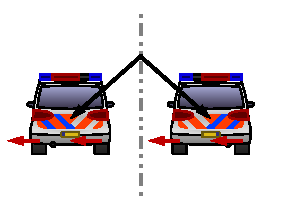
\includegraphics[scale=2]{fig/6.3.pdf}
    \caption{图中的两辆车互为镜像, 都向纸面内运动, 可以发现它们的后轮的角动量是同向的。镜像有时候来解释这个问题其实是不妥的, 因为这实际上只反演了一个坐标, 但是大致是这个意思。}
    \label{fig:6.3}
\end{figure}

如果系统有空间反演对称性\footnote{镜面对称, 或者严格点说空间三个正交基反向都行。}, 也即:
\begin{equation}
    \label{eq:6.26}
    \hat{H}^\prime=\hat{H}\Rightarrow\boxed{\left[\hat{H},\hat{\Pi}\right]=0}
\end{equation}
同样的我们得到下面的宇称守恒:
\begin{equation}
    \boxed{\frac{d}{dt}\braket{\Pi}=0}
\end{equation}

\ref{eq:6.26}中的对易式也说明了始终可以取或奇或偶的$\psi_n(x)$作为一组完备基。对于一维情况, $\hat{H}$能级非简并, 故对于$V(x)$为偶函数的体系, 也即
空间反演对称的体系, 所有的定态解组成的一组正交基一定是由奇偶函数组成, 例如$\S$2-3 的简谐振子。三维情况下由于简并的普遍性, 需要额外去构造具有宇称的定态解,不过好在
氢原子求解中的$\psi_{n\ell m}$本身就是有奇偶性的。

而且宇称守恒告诉我们在空间反演对称的体系中, 偶函数随时间演化绝对不会变成奇函数。

\subsubsection*{宇称选择定则(parity selection rule)}
像$\hat{\mathbf{r}}$或是$\hat{\mathbf{p}}$一样在宇称变换下反号的我们称为宇称变换下为\textbf{奇}的。再比如下面的电偶极矩算符:
\[\hat{\mathbf{p}}_e\equiv q\hat{\mathbf{r}}\]
这个算符显然是奇的, 我们来看下两个态之间的矩阵元:
\begin{equation}
    \Braket{\psi^\prime|\hat{\mathbf{p}}_e|\psi}=-\Braket{\psi^\prime|\hat{\Pi}^\dagger\hat{\mathbf{p}}_e\hat{\Pi}|\psi}=(\pm 1)(\pm 1)\Braket{\psi^\prime|\hat{\mathbf{p}}_e|\psi}
\end{equation}

显然, 当这两个态具有相同的宇称时, 矩阵元为0, 这也叫\textbf{Laporate's rule}, 与原子跃迁有紧密联系。同样的也可证明, 对于角动量算符这种\textbf{偶}的, 
两个态的宇称相反时, 它们之间的矩阵元为0.

\section{旋转对称性}
根据式\ref{eq:6.4}, 我们对$\psi(r,\theta,\phi-\varphi)$在$(r,\theta,\phi)$处作泰勒展开, 就像我们在\ref{eq:6.5}做的一样:
\begin{align*}
    \hat R_z(\varphi)\psi(r,\theta,\phi)&=\sum_{n=0}^\infty\frac{(-\varphi)^n}{n!}\left(\frac{\partial}{\partial \phi}\right)^n\psi(r,\theta,\phi)\\
    &=\sum_{n=0}^\infty\frac{\left(-i\frac{\varphi}{\hbar}\hat{L}_z\right)^n}{n!}\psi(r,\theta,\phi)\\
    &=\boxed{e^{-i\frac{\varphi}{\hbar}\hat{L}_z}}
\end{align*}
其中第二个等号我们利用了角动量算符在球坐标系下的表达, 也即\ref{eq:4.55}。所以我们说绕$z$轴的角动量是绕$z$轴的转动的生成元。很自然的我们可以想到对于一般的转动, 转动算符为:
\begin{equation}
    \boxed{
        \hat{R}_{\mathbf{n}}(\varphi)=\exp{\left[-i\frac{\varphi}{\hbar}\mathbf{n}\cdot\mathbf{L}\right]}
    }
\end{equation}
其中$\mathbf{n}$是转轴的方向向量。所以\textbf{角动量是转动的生成元}。

现在我们应该开始研究算符的转动变换了, 我们重点研究位置算符$\hat{\mathbf{r}}$。刚体力学中我们常常使用Euler角来描述转动, 所以我们不必直接研究最一般的转动, 我们只需研究$\hat{R}_x,\hat{R}_y,\hat{R}_z$下算符的变换关系即可。

首先我们来考虑绕x轴的无穷小转动:
\begin{equation}
    \hat{R}_z(\delta)=\mathrm e^{-i\frac{\delta}{\hbar}\hat{L}_x}\approx\mathbbm{1}-i\frac{\delta}{\hbar}\hat{L}_x
\end{equation}
忽略高阶小量$\mathcal{O}(\delta)$, 有\footnote{我们这里写了这么多$\approx$你可能认为最后得到的只是一个近似结果, 实际上是严格的等式。物理中这里使用$\approx$表示的是扔掉高阶小量, 你可以认为这些运算都是带上极限符号$\lim\limits_{\delta\to0}$, 只是没有明确写出来而已。在极限的语境下我们这些等式显然都是\textbf{严格成立}的。}:
\begin{align}
    \hat{\mathbf{r}}^\prime&=R_x(\delta)^\dagger\hat{\mathbf{r}}R_x(\delta)=\left(\mathbbm{1}+i\frac{\delta}{\hbar}\hat{L}_x\right)\hat{\mathbf{r}}\left(\mathbbm{1}-i\frac{\delta}{\hbar}\hat{L}_x\right)\\
    &\approx\boxed{\hat{\mathbf{r}}+i\frac{\delta}{\hbar}\left[\hat{L}_x,\hat{\mathbf{r}}\right]}
\end{align}
根据角动量算符的定义$\hat{\mathbf{L}}\equiv\hat{\mathbf{r}}\times\hat{\mathbf{p}}$, 以及基本对易式\ref{eq:4.48*}。可以得到:
\begin{equation}
    \left[\hat{L}_x,\hat{x}\right]=0,\left[\hat{L}_x,\hat{y}\right]=i\hbar z,\left[\hat{L}_x,\hat{z}\right]=-i\hbar y
\end{equation}
带入后我们将最后的结果写成矩阵形式为:
\begin{equation}
    \label{eq:6.34}
    \left(\begin{array}{l}
        \hat{x}^{\prime} \\
        \hat{y}^{\prime} \\
        \hat{z}^{\prime}
        \end{array}\right)=\left(\begin{array}{ccc}
        1 & 0 & 0 \\
        0 & 1 & -\delta \\
        0 & \delta & 1
        \end{array}\right)\left(\begin{array}{l}
        \hat{x} \\
        \hat{y} \\
        \hat{z}
        \end{array}\right)
\end{equation}

考虑完了无穷小转动, 自然要考虑有限大转动。首先注意到绕x轴转动有限大的角度$\varphi$, 相当于施加$N$次$\hat{R}_x\left(\frac{\varphi}{N}\right)$, 当$N\to\infty$时, $\frac{\varphi}{N}\to\delta$。
便可以利用\ref{eq:6.34}了, 这也是所谓的无穷大变换的方法。

具体来说我们下面要求的是:
\begin{equation}
    \lim_{N\to\infty}
    \left(\begin{array}{ccc}
        1 & 0 & 0 \\
        0 & 1 & -\frac{\varphi}{N} \\
        0 & \frac{\varphi}{N}& 1
        \end{array}\right)^N
\end{equation}
这等价于去求:
\begin{equation}
    \lim_{N\to\infty}
    \left(\begin{array}{ccc}
        1 & -\frac{\varphi}{N} \\
        \frac{\varphi}{N}& 1
        \end{array}\right)^N
\end{equation}
记这个矩阵为$\mathrm{M}$, 为了求这个幂, 将$\mathrm{M}$对角化:
\begin{equation}
    \mathrm{\Lambda}=\mathrm{S}^{-1}\mathrm{M}\mathrm{S}=\begin{pmatrix}
        1+\mathrm i\frac{\varphi}{N} &0 \\
       0 &1-\mathrm  i\frac{\varphi}{N} 
      \end{pmatrix}
\end{equation}
其中$\mathrm{S}$为:
\[
    \frac{1}{\sqrt{2}}\begin{pmatrix}
        i &1 \\
        1 &\mathrm i
       \end{pmatrix}
\]
注意到根据二项式定理:
\begin{equation}
    \left(1 \pm i \frac{\varphi}{N}\right)^{N}=\sum_{k=0}^{N}\mathrm C_N^{k}\left(\pm i \frac{\varphi}{N}\right)^{k}=\sum_{k=0}^{N} \frac{N !}{(N-k) ! N^{k}} \frac{(\pm i \varphi)^{k}}{k !}
\end{equation}
再取$N\to \infty$极限:
\begin{equation}
    \lim_{N\to\infty}\mathrm{\Lambda}^N=
    \begin{pmatrix}
        e^{i\varphi} &0 \\
        0 &e^{-i\varphi}
    \end{pmatrix}
    =\lim_{N\to\infty}\mathrm{S}^{-1}\mathrm{M}^N\mathrm{S}
\end{equation}
最后得到对于有限大转动\ref{eq:6.34}应改写为:
\begin{equation}
    \left(\begin{array}{l}
        \hat{x}^{\prime} \\
        \hat{y}^{\prime} \\
        \hat{z}^{\prime}
        \end{array}\right)=\left(\begin{array}{ccc}
        1 & 0 & 0 \\
        0 & \cos\varphi & -\sin\varphi \\
        0 & \sin\varphi & \cos\varphi
        \end{array}\right)\left(\begin{array}{l}
        \hat{x} \\ 
        \hat{y} \\
        \hat{z}
        \end{array}\right)
\end{equation}
同样的对于绕y轴和z轴的转动, 上面的矩阵应该改为:\footnote{一定要注意绕y轴转动的那个矩阵, $-\sin\phi$在左下方, 和另外两个看起来不同。这是旋转矩阵比较容易记混的地方。}
\begin{equation}
    \label{eq:6.41}
    \begin{pmatrix}
        \cos\varphi & 0 & \sin\varphi \\
        0 & 1& 0 \\
        {\color{red}-\sin\varphi}& 0  & \cos\varphi
    \end{pmatrix}\quad\text{and}\quad
    \begin{pmatrix}
        \cos\varphi & -\sin\varphi& 0  \\
        \sin\varphi&  \cos\varphi  &0\\
        0 & 0& 1
    \end{pmatrix}
\end{equation}

这和我们刚体力学中接触到的转动矩阵是完全一致的, 算符$\hat{\mathbf{r}}$的旋转和矢量的旋转是一致的!这就涉及到我们下面要定义的\textbf{矢量算符了}。

附录$\S $A.5中我们定义了欧氏空间中的矢量和张量, 这里类似的, 我们可以定义矢量算符就是在旋转变换下各个分量按照$\hat{\mathbf{r}}$的方式(\ref{eq:6.34},\ref{eq:6.41})变换的算符。
等等, 这里的矩阵为何与\ref{A.7}相差一个负号?这是因为\textbf{我们这里的观点就是所谓的主动观点}, 整个系统旋转, 原先的坐标系不变, 然后再考察算符的形式。而我们在刚体力学或是附录A中使用的一般是被动形式描述, 也就是说系
统本身不变, 参照系反而旋转, 然后再看算符在新的参照系下的形式。这两种观点等价, 数学描述上显然差了个负号, 但是无伤大雅。

现在回看我们的推导, 不难发现上面的定义等价于说矢量算符$\hat{\mathbf{V}}$和角动量算符之间满足如下的对易关系:
\begin{lequation}
    \label{eq:6.42}
    \boxed{
        \left[\hat L_i,\hat V_j\right]=\mathrm{i}\hbar\epsilon_{ijk}\hat{V}_k
    }
\end{lequation}
用这个式子作为矢量算符的定义是等价的, 更便于操作和叙述。而在转动下不变的算符我们称为\textbf{标量算符}:
\begin{lequation}
    \boxed{
        \left[\hat{\mathbf L},\hat f\right]=0
    }
\end{lequation}

上一节中我们讲了算符与宇称算符之间的对易关系可以将矢量和标量分为“赝”和“真”两种, 而标量和矢量的区分方法就是利用其和角动量算符的对易关系, 整理成下表\footnote{其中$\left\{\hat A,\hat B\right\}\equiv\hat A\hat B+\hat B\hat A$.}:
\begin{center}
    \begin{tabular}{llll}
        \hline \hline & parity & rotations & examples \\
        \hline true vector $\hat{\mathbf{V}}$ & $\left\{\hat{\Pi}, \hat{V}_{i}\right\}=0$ & {$\left[\hat{L}_{i}, \hat{V}_{j}\right]=i \hbar \epsilon_{i j k} \hat{V}_{k}$} & $\hat{\mathbf{r}}, \hat{\mathbf{p}}$ \\
        pseudovector $\hat{\mathbf{V}}$ & {$\left[\hat{\Pi}, \hat{V}_{i}\right]=0$} & {$\left[\hat{L}_{i}, \hat{V}_{j}\right]=i \hbar \epsilon_{i j k} \hat{V}_{k}$} & $\hat{\mathbf{L}}$ \\
        true scalar $\hat{f}$ & {$[\hat{\Pi}, \hat{f}]=0$} & {$\left[\hat{L}_{i}, \hat{f}\right]=0$} & $\hat{\mathbf{r}} \cdot \hat{\mathbf{r}}$ \\
        pseudoscalar $\hat{f}$ & $\{\hat{\Pi}, \hat{f}\}=0$ & {$\left[\hat{L}_{i}, \hat{f}\right]=0$} & triple product\\
        \hline \hline
    \end{tabular}
\end{center}

\subsubsection*{角动量守恒}
若体系具有连续的旋转对称性, 也即各向同性, 则考虑无穷小转动下的哈密顿量不变性:
\begin{equation}
    \left[\hat{H},R_{\mathbf{n}}(\delta)\right]=\left[\hat H,\mathbbm{1}-\mathrm{i}\frac{\delta }{\hbar}\mathbf{n}\cdot\mathbf{L}\right]=-\mathrm i\frac{\delta}{\hbar}\mathbf{n}\cdot\left[\hat{H},\hat{\mathbf{L}}\right]=0
\end{equation}
还是根据\ref{广义欸费斯托定理}:
\begin{equation}
    \frac{d}{dt}\braket{\mathbf{L}}=\frac{\mathrm i}{\hbar}\left[\hat{H},\hat{\mathbf{L}}\right]=0
\end{equation}
所以\textbf{角动量守恒是体系各向同性的直接结果}。一个很重要的例子就是中心势场问题, 对于中心势场, 下面的三个对易式是成立的:
\begin{equation*}
    \begin{array}{l}
    {\left[\hat{H}, \hat{L}^{2}\right]=0,} \\
    {\left[\hat{H}, \hat{L}_{z}\right]=0,} \\
    {\left[\hat{L}_{z}, \hat{L}^{2}\right]=0.}
    \end{array}
\end{equation*}

实际上, $\hat{H},\hat{L}_z, \hat{L}^2$构成了一个CSCO, 这也是为什么我们选用三个表征着三个算符的本征值的量子数$n\ell m $来描述氢原子系统的原因, 这三个量子数就唯一确定了一个定态, 
体系一般的态是这些定态的叠加态。

\section{简并与对称}
事实上, 量子力学中绝大部分的能级简并的原因都可以归结为体系具有某种对称性。\footnote{如果不是因为对称, 我们称为\textbf{偶然简并(accidental degeneracy)}。}
这部分要彻底解释清楚需要利用群表示论的相关工具, 这里先挖个坑, 先简短的做个介绍。

根据前面几节的讨论, 我们已经大致上明白对称性都对应一个幺正算符, 体系的哈密顿算符与某个与对称性有关的幺正算符对易, 那么体系就具有这种对称性。如果$\ket{\psi}$是$\hat{H}$的关于能量$E$的
本征矢, 即:
\[\hat{H}\ket{\psi}=E\ket{\psi}\]
设体系具有$\hat{Q}$的对称性, 根据$\hat{H}\hat{Q}=\hat{Q}\hat{H}$:
\begin{equation}
    \label{eq:6.46}
    \hat{H}\left(\hat{Q}\ket{\psi}\right)=\hat{Q}\hat{H}\ket{\psi}=E\hat{Q}\ket{\psi}
\end{equation}
故$\ket{\psi^\prime}=\hat{Q}\ket{\psi}$也是本征值为$E$的本征态, 很明显这时的简并就可以解释为体系的某种对称性了。

我们拿一个经典的开普勒问题来类比解释, 开普勒问题的一般解是圆锥曲线, 我们考虑椭圆解, 解的能量由半长轴唯一确定:
\begin{equation}
    \label{eq:6.47}
    E=-\frac{GMm}{2a}
\end{equation}

有心力场是具有旋转对称性的, 这也是开普勒第二定律(面积定律)的角动量守恒的原因。如果我们已知体系的某个能量为$E$的解, 那么我们将体系转动一个角度\footnote{或者用被动观点, 参考系反方向转动}, 这也是算符$\hat{R}$的作用。
显然这时轨道的取向改变了, 但是它还是开普勒问题的解。量子力学的语言就是$\ket{\psi}$是体系的解, 那么$\ket{\psi^\prime}$也是体系的解。更重要的是由于旋转是保长变换, 所以半长轴不变, 根据\ref{eq:6.47}, 这两个解对应同一个能量!
这不正好就类似于量子力学中的简并吗?!我们还知道有心力场是具有各向同性的, 所以实际上有无限多个轨道取向, 它们都对应同一个轨道能量(\ref{fig:6.4})。换成量子力学的语言就是$\ket{\psi},\hat{Q}\ket{\psi},\hat{Q}^2\ket{\psi}\ldots$均对应同一个能量, 也就是说看来连续的对称性始终会
带来无限多的简并度。

\begin{figure}[htbp]
    \centering
    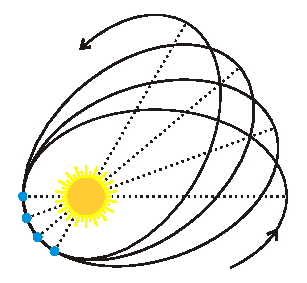
\includegraphics[scale=1.2]{fig/6-4.pdf}
    \caption{这是行星轨道进动的图, 这里是想说明椭圆轨道的多种不同取向}
    \label{fig:6.4}
\end{figure}   

经典力学中确实是这样, 但是量子力学中就不一样了, 在经典力学中, 如果两个态相同, 那么它们必须完全一致, 但是在量子力学中它们可以相差一个相因子, 即我们认为$\ket{\psi}$和$\mathrm e^{\mathrm{i}\theta}\ket{\psi}$代表的是同一个物理状态, 这也是为什么我们简并度数的是
特征空间的维数, 也就是最大线性无关组的本征矢个数。如果\ref{eq:6.46}中的$\ket{\psi}$是$\hat{Q}$的本征矢, 根据$\ket{Q}$的幺正性:
\begin{equation}
    \ket{\psi^\prime}=\hat{Q}\ket{\psi}=\mathrm e^{\mathrm{i}\theta}\ket{\psi}
\end{equation}

显然这种情况下对称性就无法带来能级的简并了, 这一点和经典力学有很大的不同。事实上, 如果体系仅仅只是拥有一个对称性, 那么显然, 我们可以取$\hat{H}$和$\hat{Q}$的共同本征矢构成的完备正交归一基, 这个时候$\hat{H}$的简并性和
体系的对称性没有一丁点关系, 因为这个基底的所有右矢都是$\hat{Q}$的本征矢, $\hat{Q}$作用在其上并不会产生“新”的$\hat{H}$的本征矢, 也就是说对称性对$\hat{H}$任何一个本征空间的维数都没有贡献。

我们证明过一维问题下束缚态能级都是非简并的, 比如一维谐振子模型, 显然他是有宇称的。但$\hat{Pi}$并没有对能级的简并有贡献, 从谐振子的定态解我们就可以看出其或奇或偶。$\hat{Pi}$作用在这些态上面只会
多出一个$\pm 1 $的相位因子, 不会产生额外的简并。

\begin{proposition}{能级简并和对称性的联系}
    体系的多个互不对易的对称性是大多数\footnote{这里写“大多数”意思是排除体系的偶然简并}能级简并的原因。
\end{proposition}

假设体系有两种对称性, $\hat{A}$和$\hat{B}$, 但是$\left[\hat{A},\hat{B}\right]\neq 0$.我们可以选取一组由$\hat{H}$和$\hat{A}$的共同本征矢构成的完备正交基$\{\psi_n\}$:
\begin{equation}
    \hat{H}\ket{\psi_n}=E_n\ket{\psi_n},\hat{Q}\ket{\psi_n}=q_n\ket{\psi_n}
\end{equation}
按照前面的解释, 简并性自然不能归咎于对称性A了, 但是设:
\[\ket{g_n}\equiv\hat{B}\ket{\psi_n}\]

如果对称性B也无法带来简并, 那么只能说所有的$\ket{\psi_n}$也都是$\ket{B}$的本征矢, 也就是说存在一个$\hat{H},\hat{A},\hat{B}$的共同本征矢构成的完备正交基, 而这必须要求三者两两简并\footnote{对易算符存在一组共同本征矢构成的正交基逆命题也是成立的, 且更容易证明, 扩展到多个算符两两对易的情况也可证明。此命题就像在第三章提到过的, 非常重要, 如果不关注证明细节就当公理吧。}。
与$\left[\hat{A},\hat{B}\right]\neq 0$矛盾, 所以这个时候能级简并就可以由体系的对称性来解释了。

最后附上一个例子, 我们将用旋转对称性来解释氢原子磁量子数的$2\ell+1$种不同取值(简并)。

\begin{thinknote}
    氢原子的有心力场具有三个轴方向的旋转对称性, 也即各向同性。$\ket{\psi_{n\ell m}}$的能级简并重点就在于$L_x,L_y,L_z$互不对易(式\ref{eq:4.48})!
    \[\left[\hat{H},\mathbf{L}\right]=0\Rightarrow\left[\hat{H},L_\pm\right]=0\]
    设$\ket{\psi_{n\ell m}}$是$\hat{H}$的本征矢, 对应的能量为$E_n$:
    \[\hat{H}\ket{\psi_{n\ell m}}=E_n\ket{\psi_{n\ell m}}\]
    根据Hamilton与$L_\pm$的对易性得:
    \[\hat{H}\left(L_\pm\ket{\psi_{n\ell m}}\right)=E_n L_\pm\ket{\psi_{n\ell m}}\]
    再根据:
    \[L_\pm \ket{\psi_{n\ell m}}=\hbar\sqrt{\ell(\ell+1)-m(m\pm 1)}\ket{\psi_{n\ell m+1}}\]
    得出:
    \[\hat{H}\left(L_\pm\ket{\psi_{n\ell m+1}}\right)=E_n L_\pm\ket{\psi_{n\ell m+1}}\]
    而$|m|>\ell$时, 上式退化为$0=0$平凡成立。这也就用各向同性解释了$\psi_n\ell m$磁量子数的简并, 而角量子数的简并是因为势能的反比例形式的额外对称性
    造成的。
\end{thinknote}

\section{旋转选择定则}
我们前面讲了宇称选择定则, 大致就是在计算矩阵元时, 因为算符和宇称算符具有一定的对易关系, 我们可以在计算前就提前确定一些为0的元素, 从而简化计算。这里我们要讲的
旋转选择定则实际上是研究当算符和角动量算符具有一定关系的时候\footnote{当然, 这实际上就是与小角度转动$\hat{R}(\delta)$之间的对易关系}, 矩阵元为0的一些条件。我们下面的讨论不涉及宇称, 讨论标量算符和矢量算符的一般结论, 所以对于真赝
矢量(标量)都是适用的。\footnote{我们这些讨论最后可以进化为一个量子力学中非常重要的Wigner-Eckart定理}
\subsection{标量算符的选择定则}
根据标量算符的定义:
\begin{equation}
    \left[\hat{\mathbf{L}},\hat{f}\right]=0\Rightarrow\begin{cases}
        \left[\hat{L_\pm},\hat{f}\right]=0\\
        \left[\hat{L}_z,\hat{f}\right]=0\\
        \left[\hat{L}^2,\hat{f}\right]=0
    \end{cases}
\end{equation}

下面我们将使用符号$\ket{\alpha\ell m}$来表示某个量子态, $\alpha,\ell,m$三个数是描述这个态相应的量子数, 所有可能取值的集合就构成了体系量子态的一组完备正交归一
基底。前面我们使用$\ket{n\ell m}$去描述氢原子, 这实际上是选取了$\hat{H},L^2,L_z$构成的CSCO。这里我们使用$\alpha $而不是$n$去标记就是表明我们完全可以依照研究内容的不同, 方便的取
$\hat{Q},L_z,L^2$作为CSCO, $\hat{Q}$不必再是哈密顿量。$\ket{\alpha\ell m}$是它们的共同本征矢, 所以关于角动量的那些代数结构结论我们可以继续用。

根据$\left[\hat{L}_z,\hat{f}\right]=0$:
\begin{align*}
    &\Braket{\alpha^\prime   \ell^\prime   m^\prime  |\left[\hat{L}_z,\hat{f}\right]|\alpha \ell m}=0\\
    \Rightarrow&\Braket{\alpha^\prime   \ell^\prime   m^\prime  |\hat{L}_z\hat{f}|\alpha \ell m}-\Braket{\alpha^\prime   \ell^\prime   m^\prime  |\hat{f}\hat{L}_z|\alpha \ell m}=0\\
    \Rightarrow&\left(m^\prime-m\right)\Braket{\alpha^\prime   \ell^\prime   m^\prime  |\hat{f}|\alpha \ell m}=0
\end{align*}

注意上面最后一个等式的得到我们利用了\ref{eq:4.53}, $\hat L_z$的厄米性以及$m\in \mathbb{R}$。根据上面的推导, 当且仅当$m=m^\prime$时矩阵元$\braket{\alpha^\prime   \ell^\prime   m^\prime  |\hat{f}|\alpha \ell m}$
\uwave{可能}不为0。同样的, 根据$\left[\hat{L}^2,\hat{f}\right]=0$:
\begin{equation}
    \left[\ell^\prime(ell^\prime +1)-\ell(\ell+1)\right]\Braket{\alpha^\prime   \ell^\prime   m^\prime  |\hat{f}|\alpha \ell m}=0
\end{equation}

这次我们得到的是当且仅当$\ell=\ell^\prime$时矩阵元可能不为0。\footnote{当然上面的方程如果$\ell^\prime=-(\ell+1)$时也会得到trivial的$0=0$, 但是显然根据角量子数的可能取值, 这个解需要舍弃。}
继续考虑$\left[\hat{L}_\pm,\hat{f}\right]=0$:
\begin{align*}
    &\Braket{\alpha^\prime   \ell^\prime   m^\prime  |\left[\hat{L}_\pm,\hat{f}\right]|\alpha \ell m}=0\\
    \Rightarrow&\Braket{\alpha^\prime   \ell^\prime   m^\prime  |\hat{L}_\pm\hat{f}-\hat{f}\hat{L}_\pm|\alpha \ell m}=0\\
    \Rightarrow&\left(L_\mp\ket{\alpha^\prime   \ell^\prime   m^\prime  }\right)^\dagger\hat{f}\ket{\alpha\ell m}-\Braket{\alpha^\prime   \ell^\prime   m^\prime  |\hat{f}\hat{L}_\pm|\alpha\ell m}\\
    \Rightarrow&\sqrt{\ell^\prime(\ell^\prime+1)-m^\prime(m^\prime\mp 1)}\Braket{\alpha^\prime   \ell^\prime   (m^\prime\mp 1)  |\hat{f}|\alpha \ell m}\\
    &-\sqrt{\ell(\ell+1)-m(m\pm 1)}\Braket{\alpha^\prime   \ell^\prime   m^\prime  |\hat{f}|\alpha \ell (m\pm 1)}
\end{align*}

再根据我们前面的两个结论只有在$m^\prime=m+1 \wedge \ell^\prime=\ell$的情况下, 上面的等式不是trivial的$0=0$。在这种情况下可以继续得到:
\begin{equation}
    \Braket{\alpha^\prime\ell m|\hat{f}|n\ell m}=\Braket{\alpha^\prime\ell (m+1)|\hat{f}|n\ell (m+1)}
\end{equation}

上面的式子可以反复迭代, 而且结合磁量子数取值的步长为1, 所以上面的式子说明的实际上是$\Braket{\alpha^\prime \ell m|\hat{f}|\alpha\ell m}$的取值与m无关\footnote{一定要注意在这个结论的适用条件下, 矩阵元前后的两个态仅仅是$\alpha$这个量子数有区别},所以这个时候我们可以使用统一的一个不包含m 的符号来指代这一系列相等的矩阵元:
\begin{equation}
    \label{eq:6.53}
    \Braket{\alpha^\prime \ell \|\hat{f}\|\alpha\ell }\equiv\Braket{\alpha^\prime \ell -\ell|\hat{f}|\alpha\ell -\ell}=\cdots=\Braket{\alpha^\prime \ell \ell|\hat{f}|\alpha\ell \ell}
\end{equation}
这里使用了双竖线来区分, 称为约化矩阵元(reduced matrix element)。

结合所有上面的三个结论, 可以发现实际上它们可以写成下面的形式:
\begin{lequation}
    \label{eq:6.54}
    \boxed{\Braket{\alpha^\prime\ell^\prime m^\prime|\hat{f}|\alpha \ell m}=\delta_{\ell\ell^\prime}\delta_{mm^\prime}\Braket{\alpha^\prime \ell^\prime \|\hat{f}\|\alpha\ell }}
\end{lequation}
下面举个例子来说明如何利用这个定理来简化计算:\footnote{啰嗦一句, 下面最后的计算使用的是球坐标计算, 这个表象下$\hat{r}^2$算符就是直接波函数乘上$r^2$。如果硬是要使用直角坐标计算, 那么这个表象下相当于波函数乘上$x^2+y^2+z^2$}
\begin{thinknote}
    下面是氢原子系统电子的某个轨道量子态, 试求这个态下的$\braket{r^2}$:
    \begin{equation}
        \ket{\psi}=\frac{1}{\sqrt{2}}\left(\ket{200}-i\ket{211}\right)
    \end{equation}
    根据定义, 我们实际上要计算的是矩阵元$\Braket{\psi|\hat{r}^2|\psi}$, 而$\hat{r}^2$是一个标量算符。
    \begin{align*}
        \Braket{r^2}=&\frac{1}{2}\left(\bra{200}+i\bra{211}\right)\hat{r}^2\left(\ket{200}-i\ket{211}\right)\\
        =&\frac{1}{2}\left(\Braket{200|\hat{r^2}|200}-i\Braket{200|\hat{r^2}|211}+i\Braket{211|\hat{r^2}|200}\right.\\
        &\left.+\Braket{211|\hat{r^2}|211}\right)
    \end{align*}
    根据\ref{eq:6.54}:
    \begin{equation}
        \Braket{200|\hat{r^2}|211}=\Braket{211|\hat{r^2}|200}=0
    \end{equation}
    而计算另外两个实际上是计算约化矩阵元:
    \[\Braket{20\|\hat{r^2}\|20}\quad \text{and}\quad \Braket{21\|\hat{r^2}\|21}\]
    我们可以都选取$m=0$来简化约化矩阵元的计算, 详细计算过程贴在这里了:
    \begin{align*}
        \Braket{20\|\hat{r^2}\|20}&=\Braket{200|\hat{r^2}|200}\\
        &=\int r^{2}\left|\psi_{200}(r)\right|^{2} d^{3} \mathbf{r} \\
        &=\int_{0}^{\infty} r^{4}\left|R_{20}(r)\right|^{2} d r \int\left|Y_{0}^{0}(\theta, \phi)\right|^{2} d \Omega \\
        &=\int_{0}^{\infty} r^{4} \frac{1}{2 a^{3}}\left(1-\frac{1}{2} \frac{r}{a}\right)^{2} e^{-r / a} d r \\
        &=\boxed{42 a^{2} }
    \end{align*}
    \begin{align*}
        \Braket{21\|\hat{r^2}\|21}&=\Braket{210|\hat{r^2}0|210}\\
        &=\int r^{2}\left|\psi_{210}(r)\right|^{2} d^{3} \mathbf{r} \\
        &=\int_{0}^{\infty} r^{4}\left|R_{21}(r)\right|^{2} d r \int\left|Y_{1}^{0}(\theta, \phi)\right|^{2} d \Omega\\
        &=\int_{0}^{\infty} r^{4} \frac{1}{24 a^{3}} \frac{r^{2}}{a^{2}} e^{-r / a} d r\\
        &=\boxed{30 a^{2}}
    \end{align*}
    所以最终的结果为$36a^2$, $a$是玻尔半径。
\end{thinknote}

\subsection{矢量算符的选择定则}
矢量算符比标量算符麻烦多了, 首先类似于$\hat L_\pm$, 我们定义$\hat V_\pm$:
\begin{equation}
    \hat V_\pm\equiv\hat{V}_x\pm i \hat{V}_x
\end{equation}
根据\ref{eq:6.42}, 我们有如下的对易关系:
\begin{align}
    {\left[\hat{L}_{z}, \hat{V}_{z}\right] } &=0 \label{eq:6.57}\\
    {\left[\hat{L}_{z}, \hat{V}_{\pm}\right] } &=\pm \hbar \hat{V}_{\pm} \label{eq:6.58} \\
    {\left[\hat{L}_{\pm}, \hat{V}_{\pm}\right] } &=0 \label{eq:6.59} \\
    {\left[\hat{L}_{\pm}, \hat{V}_{z}\right] } &=\mp \hbar \hat{V}_{\pm} \label{eq:6.60} \\
    {\left[\hat{L}_{\pm}, \hat{V}_{\mp}\right] } &=\pm 2 \hbar \hat{V}_{z} \label{eq:6.61}
\end{align}

然后我们要干的活儿就和上一节一样了, 还是把这些对易关系夹在中间。\ref{eq:6.57}和\ref{eq:6.58}的计算比较简单, 可以据此得到:
\begin{align}
    \Braket{\alpha^{\prime} \ell^{\prime} m^{\prime}|\hat{V}_{+}| \alpha \ell m}  & = 0 \quad \text { unless } m^{\prime}  = m+1\label{eq:6.63}\\
    \Braket{\alpha^{\prime} \ell^{\prime} m^{\prime}|\hat{V}_{z}| \alpha \ell m}  & = 0 \quad \text { unless } m^{\prime}  = m\label{eq:6.64}\\
    \Braket{\alpha^{\prime} \ell^{\prime} m^{\prime}|\hat{V}_{-}| \alpha \ell m}  & = 0 \quad \text { unless } m^{\prime}  = m-1 \label{eq:6.65}
\end{align}

再根据$\hat{V}_x,\hat{V}_y$与$\hat{V}_+,\hat{V}_-$之间的关系就可以将上述选择定则用于计算$\Braket{\alpha^{\prime} \ell^{\prime} m^{\prime}|\hat{V}_{x}| \alpha \ell m}$和
$\Braket{\alpha^{\prime} \ell^{\prime} m^{\prime}|\hat{V}_{y}| \alpha \ell m}$了。

比较难的是\ref{eq:6.59}$\sim$\ref{eq:6.61}的计算, 下面给出最一般的结论, 和最最一般的Wigner-Eckart定理已经非常相近了\footnote{这一节{\itshape Griffiths}书后面的习题有一个\uwave{验证性}证明。}:
\begin{equation}
    \label{eq:6.66}
    \boxed{
        \begin{aligned}
            \Braket{\alpha^{\prime} \ell^{\prime} m^{\prime}|\hat{V}_{+}| \alpha \ell m}  & = -\sqrt{2}C^{\ell 1 \ell^\prime}_{m 1 m^\prime}\Braket{\alpha^\prime\ell^\prime\|\mathbf{V}\|\alpha\ell}\\
            \Braket{\alpha^{\prime} \ell^{\prime} m^{\prime}|\hat{V}_{-}| \alpha \ell m}  & =  \sqrt{2}C^{\ell 1 \ell^\prime}_{m -1 m^\prime}\Braket{\alpha^\prime\ell^\prime\|\mathbf{V}\|\alpha\ell}\\
            \Braket{\alpha^{\prime} \ell^{\prime} m^{\prime}|\hat{V}_{z}| \alpha \ell m}  & =  C^{\ell 1 \ell^\prime}_{m 0 m^\prime}\Braket{\alpha^\prime\ell^\prime\|\mathbf{V}\|\alpha\ell}
        \end{aligned}
    }
\end{equation}

这里我们又遇到了CG系数$C^{j_1j_2J}_{m_1m_2M}$, 上面的式子实际上是包含了6.63, 6.64和6.65的结论的。因为CG系数仅在
\[m_1+m_2=M\quad\text{and}\quad J=(j_1+j_2),(j_1+j_2-1),\ldots,|j_1-j_2|\]
的情况下不为0, 可以用角动量合成的理论理解。态$\ket{s,m}$只能分解成那些满足上式取值的态$\ket{s_1,s_2,m_1,m_2}$的线性组合(\ref{eq:4.96})。所以那些不满足这些取值的$C^{j_1j_2J}_{m_1m_2M}$
在CG系数表里面压根没有, 也就是说它们等于0. 根据这里的讨论, 我们得出$\hat{\mathbf{V}}$的各个分量的矩阵元$\Braket{\alpha^{\prime} \ell^{\prime} m^{\prime}|\hat{V}_{i}| \alpha \ell m} $
\textbf{不为0}的条件是:
\begin{equation*}
    \boxed{
        \Delta \ell = 0,\pm 1\quad \text{and}\quad \Delta m = 0,\pm 1 
    }
\end{equation*}

特别注意, 这里的约化矩阵元$\Braket{\alpha^\prime\ell^\prime\|\mathbf{V}\|\alpha\ell}$是一个与$m,m^\prime$无关的量, 但是并不是和\ref{eq:6.53}一般的定义, 也就是
说\textbf{不能通过随便选取$m$来计算它}。详细的定义比较复杂, 但是我们可以根据\ref{eq:6.66}来间接计算出它, 比如根据第三个式子, 我们只要按照通常的方法计算矩阵元
$\Braket{\alpha^{\prime} \ell^{\prime} m^{\prime}|\hat{V}_{z}| \alpha \ell m} $, 然后再乘上一个系数就可以了。

最后, 因为$C^{\ell 0\ell^\prime}_{m0m^\prime}=\delta_{mm^\prime}\delta_{\ell\ell^\prime}$, 所以我们可以把标量算符的选择定则\ref{eq:6.54}写成类似的形式:
\begin{equation}
    \boxed{\Braket{\alpha^\prime\ell^\prime m^\prime|\hat{f}|\alpha \ell m}=C^{\ell 0\ell^\prime}_{m0m^\prime}\Braket{\alpha^\prime \ell^\prime \|\hat{f}\|\alpha\ell }}
\end{equation}

\section{时间平移对称性}
按照空间平移算符的定义, 或许时间平移算符就是将态在时间轴上平移, 也就是说得到演化一段时间后的态$\ket{\psi(t+t_0)}$。既然谈到态的演化, 我们就更应该用薛定谔方程来详细引入:
\[i\hbar\frac{\partial}{\partial t}\ket{\psi(t)}=\hat{H}\ket{\psi(t)}\]
这个方程唯一确定了态随时间的演化, 我们如此定义\textbf{时间演化算符}:
\begin{equation}
    \label{eq:6.68}
    \hat{U}(t,t_0)\ket{\psi(t_0)}=\ket{\psi(t)}
\end{equation}
我们一般便利的取$t_0=0$下面的推导中我们简写算符为$\hat{U}(t)$。

我们在位置表象下用波函数来表示\ref{eq:6.68}, 并把波函数对$t$作麦克劳林展开\footnote{并不是所有函数都能随便展开成幂级数形式, 对应的还要考虑收敛域, 所以下面我们得到了时间演化算符的形式严格意义上来说\textbf{并不是普适的}。这篇论文研究了这个问题:\DOI{10.1119/1.4985723}。物理人用起来实际上也很少有问题, 彻底严谨化那套是数学家玩的。}:
\begin{align*}
    \hat{U}(t)\Psi(\mathbf{r},0)&=\Psi(\mathbf{r},t)\\
    &=\sum_{n=0}^\infty \frac{t^n}{n!}\left.\frac{\partial^{n}}{\partial t^{n}} \Psi(\mathbf{r}, t)\right|_{t=0}
\end{align*}
如果$\hat{H}$不显含时间, 根据薛定谔方程:
\begin{equation}
    \left.\frac{\partial^{n}}{\partial t^{n}} \Psi(\mathbf{r}, t)\right|_{t=0}=\left(\frac{\hat{H}}{i\hbar}\right)^n\Psi(\mathbf{r},0)
\end{equation}
代入上面的推导, 我们便得到时间演化算符的具体形式:
\begin{equation}
    \label{eq:6.70}
    \boxed{\hat{U}(t)=\exp \left[-\frac{i t}{\hbar} \hat{H}\right]}
\end{equation}

这个玩意和薛定谔方程是等价的, 都唯一确定了量子态在给定初值下的演化。对一个体系, 如果我们得到了其态空间内的一组完备基, 不妨就用$\ket{\psi}$标记\footnote{这里我们选择了最方便的形式, 只有一个指标来标记基底。但实际上可以有多个指标, 这与我们CSCO的选取有关, 比如我们接触过的$\ket{n\ell m}$}。
我们可以把初态写成这些的线性组合:
\[\ket{\Psi(0)}=\sum_{n=1}^{\infty}c_n\ket{\psi_n}\]
则态之后的演化可以根据时间演化算符的作用得到:
\[\ket{\Psi(t)}=\hat{U}(t)\ket{\Psi(0)}=\sum_{n=1}^{\infty}c_ne^{-i\frac{t}{\hbar}\hat{H}}\ket{\psi_n}\]
如果我们取的就是能量表象, 根据定态方程, 上式可以便为:
\[\ket{\Psi(t)}=\sum_{n=1}^{\infty}c_ne^{-i\frac{t}{\hbar}E_n}\ket{\psi_n}\]
我们再次得到了前面通过空间时间分离变量得到的结论。

\subsection{薛定谔/海森堡绘景}
不难发现, 时间演化算符又是一个幺正算符。按照套路, 我们现在应该去研究一般的算符在这个算符下的幺正变换了, 即$\hat Q^\prime=\hat{U}^\dagger\hat{Q}\hat{U}$。前面的这些变换后的算符都可以解释为系统在平移或者旋转这些空间变换之后算符的形式。那这里应该解释成体系在时间演化下
算符的变化吗?也即算符随时间的演化?可前面我们说一个系统随时间演化时位置动量算符都不随时间变化啊?!这里我们就需要引入\textbf{薛定谔绘景(Sch\"odinger picture)}和\textbf{海森堡绘景(Heisenberg picture)}了。

回到最初我们说对算符的“平移”,“旋转”操作。对于某个力学量$Q$, 我们要计算体系在平移前后力学量的平均值:
\begin{align*}
    \text{before}:&\braket{Q}=\Braket{\psi|\hat{Q}|\psi}\\
    \text{after}:&\braket{Q}=\Braket{\psi^\prime|\hat{Q}|\psi^\prime}=\Braket{\psi|T^\dagger\hat{Q}T|\psi}
\end{align*}

不难发现, 我们要计算平移后力学量的平均值, 一种很自然的观点就是算符还是那个算符, 但是体系给平移一下;另一种观念就是态矢我们不变, 还是用原来那个态矢, 但是
我们计算的时候中间“夹”的那个算符用“平移后的算符”$\hat{Q}^\prime=T^\dagger\hat{Q}T$。把这个空间平移换成时间平移, 我们前面实际上一直使用的都是薛定谔绘景, 
回忆一下计算某个力学量在某个时刻的平均值我们是这样做的:
\[\braket{Q}=\Braket{\psi(t)|\hat{Q}_S|\psi(t)}\]

动量、位置算符这些本身都不随时间变化, 态矢量按照薛定谔方程随时间演化, 从而导致力学量的演化。为了和后面的海森堡绘景区分, 我们为对应的力学量加上了下标S。

态矢随时间的演化可以用时间演化算符确定, 将\ref{eq:6.68}代入上式, 我们得到:
\[\braket{Q}=\Braket{\psi(0)|\left(\hat{U}^\dagger\hat{Q}_S\hat{U}\right)|\psi(0)}\]
我们定义:
\begin{equation}
    \label{eq:6.71}
    \hat{Q}_H(t)\equiv\hat{U}^\dagger(t)\hat{Q}_S\hat{U}(t)
\end{equation}

现在我们计算$\braket{Q}$采取态矢量不动(计算时始终用初态$\ket{\psi(0)}$), 而算符随着时间演化的方法。这两个绘景就是描述同一个问题的两种方法, 只是看到底把时间演化归咎于态本身还是力学量算符而已。某种意义上来说, 海森堡绘景就是
\textbf{态空间基矢运动, 态矢不动};薛定谔绘景就是\textbf{基矢不动, 态矢运动}。就像是一个时钟, 我们可以表针不动表盘运动, 也可以表盘运动表针不动, 但都指向同一个正确的时间\footnote{当然还可以表针表盘一起动, 这是相互作用绘景(Dirac绘景)。}。

采用薛定谔绘景时\footnote{后面都用这个绘景}, 重点就是利用薛定谔方程计算态矢随时间的变化。而对应的海森堡绘景, 这个时候$\hat{Q}_H(t)$的演化满足\textbf{海森堡方程}, 下面我们
对于哈密顿量和力学量$Q$不显含时间的情况加以说明。\footnote{对于哈密顿算符显含时间的一般海森堡方程为:\[i \hbar \frac{d}{d t} \hat{Q}_{H}(t)=\left[\hat{Q}_{H}(t), \hat{H}_{H}(t)\right]+\hat{U}^{\dagger} \frac{\partial \hat{Q}}{\partial t} \hat{U}\]}

将\ref{eq:6.71}两边对时间微分:
\begin{equation}
    \label{eq:6.72}
    \frac{d\hat{Q}_H}{dt}=\frac{d\hat{U}^\dagger}{dt}\hat{Q}_S\hat{U}+\hat{U}^\dagger\hat{Q}_S\frac{d\hat{U}}{dt}
\end{equation}
再根据\ref{eq:6.70}以及附录$\S$B.6相关内容:
\begin{equation}
    \frac{d\hat{U}}{dt}=\frac{\hat{H}}{i\hbar}\hat{U}
\end{equation}
代入到\ref{eq:6.72}得:
\begin{align*}
    i\hbar\frac{d\hat{Q}_H}{dt}&=\hat{U}^\dagger\hat{Q}_S\hat{H}\hat{U}-\hat{H}\hat{U}^\dagger\hat{Q}_S\hat{U}\\
    &=\left[\hat{U}^\dagger\hat{Q}_S\hat{U},\hat{H}\right]\equiv\left[\hat{Q}_H,\hat{H}\right]
\end{align*}

注意第二个等号我们利用了$\left[\hat{H},\hat{U}\right]=0$。其实和玩意和反复提及的\ref{广义欸费斯托定理}形式很像是吧。利用它, 我们就可以更为便利的去计算某个具体系统的
$\hat{x}_H$等等, 我们下面以谐振子为例。\footnote{注意下面的推导中, 利用了$\hat{Q}_H(0)=\hat{Q}_S$去表达结果}
\[\hat{H}=\frac{\hat{p}^2}{2m}+\frac{1}{2}m\omega^2x^2\]
\begin{thinknote}
    首先我们直接按照定义来求:
    \[\hat{x}_H(t)=\mathrm e^{i\frac{t}{\hbar}\hat{H}}\hat{x}\mathrm e^{-i\frac{t}{\hbar}\hat{H}}\]
    直接这么算肯定很难, 我们得充分利用已知结论, 利用升降阶算符, 我们可以把位置算符写成:
    \[\hat{x}=\sqrt{\frac{\hbar}{2m\omega}}\left(\hat{a}_++\hat{a}_-\right)\]
    而算符最终肯定是要作用到态矢量上面的, 我们不妨就选取能量表象下的$\ket{\psi_n}$, 由于它们张成了体系的态空间, 所以只要求出$\hat{x}_H$对每个$\ket{\psi_n}$都成立, 那也就顺理成章的对所有的态都成立了。
    \begin{align*}
        \hat{x}_H(t)\ket{\psi_n}&=\mathrm e^{i\frac{t}{\hbar}\hat{H}}\sqrt{\frac{\hbar}{2m\omega}}\left(\hat{a}_++\hat{a}_-\right)\mathrm e^{-i\frac{t}{\hbar}E_n}\ket{\psi_n}\\
        &=\sqrt{\frac{\hbar}{2m\omega}}\mathrm e^{-i\frac{t}{\hbar}E_n}\mathrm e^{i\frac{t}{\hbar}\hat{H}}\left(\sqrt{n+1}\ket{\psi_{n+1}}+\sqrt{n}\ket{\psi_{n-1}}\right)\\
        &=\sqrt{\frac{\hbar}{2m\omega}}\mathrm e^{-i\frac{t}{\hbar}E_n}\left[\sqrt{n+1}\ket{\psi_{n+1}}e^{i\frac{t}{\hbar}E_{n+1}}+\sqrt{n}\ket{\psi_{n-1}}e^{i\frac{t}{\hbar}E_{n-1}}\right]\\
        &=\sqrt{\frac{\hbar}{2 m \omega}}\left[\sqrt{n+1} e^{i \omega t} \ket{\psi_{n+1}}+\sqrt{n} e^{-i \omega t} \ket{\psi_{n-1}}\right]
    \end{align*}
    上式第一个等号利用了定态方程, 第二个等号利用了递推关系\ref{eq:2.21}, 最后一个等号利用了能级$E_n=(n+\frac{1}{2})\omega\hbar$。综上,得到:
    \[\hat{x}_{H}(t)=\sqrt{\frac{\hbar}{2 m \omega}}\left[e^{i \omega t} \hat{a}_{+}+e^{-i \omega t} \hat{a}_{-}\right]\]
    利用产生湮灭算符的定义, 将上式利用$\hat{x},\hat{p}$亦可重新写为:
    \[\hat{x}_{H}(t)=\hat{x}_{H}(0) \cos (\omega t)+\frac{1}{m \omega} \hat{p}_{H}(0) \sin (\omega t)\]
    其实使用海森堡方程, 上面的结论可以很快的得出, 我们下面对一般的势场进行推演:
    \begin{equation}
        \begin{aligned}
            \frac{d}{d t} \hat{x}_{H} &=\frac{1}{i \hbar}\left[\hat{x}_{H}, \hat{H}\right]=\frac{1}{i \hbar}\left[\hat{U}^{\dagger} \hat{x} \hat{U}, \hat{H}\right] \\
            &=\frac{1}{i \hbar}\left(\hat{U}^{\dagger} \hat{x}\underbrace{\left[\hat{U}, \hat{H}\right ]}_{0}+\hat{U}^{\dagger}[\hat{x}, \hat{H}] \hat{U}+\underbrace{\left[U^{\dagger}, \hat{H}\right]}_{0} \hat{x} \hat{U})\right)\\
            &=\frac{1}{i \hbar} \hat{U}^{\dagger}\left[\hat{x}, \frac{\hat{p}^{2}}{2 m}+V(x)\right] \hat{U} \\
            &=\frac{1}{i \hbar} \hat{U}^{\dagger}(\frac{1}{2 m}\left[\hat{x}, \hat{p}^{2}\right]+\underbrace{[\hat{x}, V]}_{0}) \hat{U} \\
            &=\frac{1}{i \hbar} \hat{U}^{\dagger} \frac{1}{2 m}(\hat{p} \underbrace{[\hat{x}, \hat{p}]}_{i \hbar}+[\hat{x}, \hat{p}] \hat{p}) \hat{U} \\
            &=\frac{1}{m} \hat{U}^{\dagger} \hat{p} \hat{U}=\frac{1}{m} \hat{p}_{H}(t) 
        \end{aligned}
    \end{equation}
    同理, 对于$\hat{p}_H(t)$:
    \begin{equation}
        \begin{aligned}
            \frac{d}{d t} \hat{p}_{H} &=\frac{1}{i \hbar} \hat{U}^{\dagger}\left[\hat{p}, \frac{\hat{p}^{2}}{2 m}+V\right] \hat{U} \\
            &=\frac{1}{i \hbar} \hat{U}^{\dagger}\left(\underbrace{\left[\hat{p}, \frac{\hat{p}^{2}}{2 m}\right]}_{0}+[\hat{p}, V(x)]\right) \hat{U} \\
            &=\frac{1}{i \hbar} \hat{U}^{\dagger}\left(-i \hbar \frac{d V}{d x}\right) \hat{U}\equiv \left(-\frac{d V}{d x}\right)_{H}(t)
        \end{aligned}
    \end{equation}
    写在一起便是
    \begin{equation}
        \boxed{m \frac{d \hat{x}_{H}}{d t}=\hat{p}_{H}(t) \quad \frac{d \hat{p}_{H}}{d t}=\left(-\frac{d V}{d x}\right)_{H}}
    \end{equation}

    \setlength\parindent{2em}这太眼熟了, 这形式上不就是经典力学里面的粒子的运动方程吗?所以海森堡方程告诉我们, 形式上, 算符的演化规律和经典力学里面的位移动量随时间的变化是一样的。
    你看我们上面的得到的$\hat{x}_H(t)$, 这不是和经典谐振子的简谐运动方程:
    \[x(t)=x(0)\cos(\omega t)+\frac{v(0)}{\omega}\sin (\omega t)\]
    形式上一模一样么?
    \hfill $\square$\par
\end{thinknote}
\subsection{能量守恒定律}
对于一般的系统, 哈密顿算符可能显含时间, 我们依旧可以定义时间演化算符:
\begin{equation}
    \label{eq:6.77}
    \ket{\Psi(t)}=\hat{U}(t,t_0)\ket{\Psi(t_0)}
\end{equation}
只是这里的$\hat{U}(t,t_0)$不再具有\ref{eq:6.70}的形式。

我们下面考察系统无限小时间内的演化, 我们再次回到坐标表象下用波函数$\Psi(\mathbf{r},t)$来写方程, 我们假设波函数始终可以对时间作泰勒展开。对于哈密顿量
显含时间的问题, 最麻烦的点就是高阶的$\frac{\partial^n}{\partial t^n}$不能用$\hat{H}$的幂表示。但没关系, 我们考虑的是无穷小演化, 高阶量都可以丢掉。
\begin{align*}
    \Psi(\mathbf{r},t_0+\delta)&=\left(1+\delta\left.\frac{\partial }{\partial t}\right|_{t=t_0}+\mathcal{O}(\delta)\right)\Psi(\mathbf{r},t)\\
    &=\left(1-\mathrm{i}\frac{\delta}{\hbar}\hat{H}+\mathcal{O}(\delta)\right)\Psi(\mathbf{r},t_0)
\end{align*}
把后面的那个高阶小量丢掉, 然后和\ref{eq:6.77}对比:
\begin{equation}
    \label{eq:6.78}
    \hat{U}(t_0+\delta,t_0)\overset{!}{=}\mathbbm{1}-i\frac{\delta}{\hbar}\hat{H}
\end{equation}
很巧, 这玩意儿我们要是直接用\ref{eq:6.70}, 展开到一阶也能得到, 但我们说过了\ref{eq:6.70}仅适用于哈密顿量不显含时间的系统。

何谓(连续的)时间平移对称性?我们用形象的语言解释就是周三和周四在同样的初始条件下做实验, 应该得到相同的结果, 仅仅只是你记录实验的初始和末尾的时间有差别而已。
转换成标准化的语言来说就是, 态矢量$\ket{\alpha}$在$t_1$时刻开始演化一个无穷小时间到$\ket{\beta}$, 那同样的条件下, $\ket{\alpha}$在$t_2$时刻开始演化一个无穷小时间也应该得到$\ket{\beta}$。
也就是说下面的式子对$\forall t_1,t_2$都成立:
\[\hat U(t_1+\delta,t_1)=\hat{U}(t_2+\delta,t_2)\]
根据\ref{eq:6.78}, 这意味着下面的等式恒成立:
\[\hat{H}(t_1)=\hat{H}(t_2)\]
这实际上也就是在说\textbf{哈密顿量不显含时间}, $\frac{\partial \hat{H}}{\partial t}=0$。再利用\ref{广义欸费斯托定理}, 我们得到:
\[\frac{d}{dt}\braket{H}=0\]
即能量守恒, 所以\textbf{时间的连续平移对称性直接导致了体系的能量守恒(Hamiltonian不显含时间)}。

这一整章我们都在讲对称性和守恒律之间的联系, 因为数学水平有限, 没有涉及到群论来更加深刻的讨论, 等后续补充。而且这章我觉得有些地方我写的也不够清楚, 有待完善。
除了连续对称性对应的守恒律, 量子力学中宇称是可观测量, 观测值为$\pm 1$, 离散的宇称变换对称性也对应了宇称守恒。这章最难以理解的估计就是选择定理了, 那东西得上群论才能彻底讲清楚,
初量的任务就是理清楚矢量算符的定义就好, 那三个转动矩阵的来历和对应的计算也很重要。
